\documentclass[12pt,letterpaper,]{book}
\usepackage{lmodern}
\usepackage{amssymb,amsmath}
\usepackage{ifxetex,ifluatex}
\usepackage{fixltx2e} % provides \textsubscript
\ifnum 0\ifxetex 1\fi\ifluatex 1\fi=0 % if pdftex
  \usepackage[T1]{fontenc}
  \usepackage[utf8]{inputenc}
\else % if luatex or xelatex
  \ifxetex
    \usepackage{mathspec}
  \else
    \usepackage{fontspec}
  \fi
  \defaultfontfeatures{Ligatures=TeX,Scale=MatchLowercase}
    \setmainfont[]{Cambria}
    \setsansfont[]{Arial}
    \setmathfont(Digits,Latin,Greek)[]{Cambria}
\fi
% use upquote if available, for straight quotes in verbatim environments
\IfFileExists{upquote.sty}{\usepackage{upquote}}{}
% use microtype if available
\IfFileExists{microtype.sty}{%
\usepackage{microtype}
\UseMicrotypeSet[protrusion]{basicmath} % disable protrusion for tt fonts
}{}
\usepackage[top=2.5cm, bottom=2.5cm, left=3cm, right=3cm]{geometry}
\usepackage{hyperref}
\PassOptionsToPackage{usenames,dvipsnames}{color} % color is loaded by hyperref
\hypersetup{unicode=true,
            pdftitle={Ecología de poblaciones silvestres},
            pdfauthor={David Martínez Cascante},
            colorlinks=true,
            linkcolor=blue,
            citecolor=blue,
            urlcolor=blue,
            breaklinks=true}
\urlstyle{same}  % don't use monospace font for urls
\usepackage{natbib}
\bibliographystyle{DAVID}
\usepackage{color}
\usepackage{fancyvrb}
\newcommand{\VerbBar}{|}
\newcommand{\VERB}{\Verb[commandchars=\\\{\}]}
\DefineVerbatimEnvironment{Highlighting}{Verbatim}{commandchars=\\\{\}}
% Add ',fontsize=\small' for more characters per line
\usepackage{framed}
\definecolor{shadecolor}{RGB}{248,248,248}
\newenvironment{Shaded}{\begin{snugshade}}{\end{snugshade}}
\newcommand{\KeywordTok}[1]{\textcolor[rgb]{0.13,0.29,0.53}{\textbf{#1}}}
\newcommand{\DataTypeTok}[1]{\textcolor[rgb]{0.13,0.29,0.53}{#1}}
\newcommand{\DecValTok}[1]{\textcolor[rgb]{0.00,0.00,0.81}{#1}}
\newcommand{\BaseNTok}[1]{\textcolor[rgb]{0.00,0.00,0.81}{#1}}
\newcommand{\FloatTok}[1]{\textcolor[rgb]{0.00,0.00,0.81}{#1}}
\newcommand{\ConstantTok}[1]{\textcolor[rgb]{0.00,0.00,0.00}{#1}}
\newcommand{\CharTok}[1]{\textcolor[rgb]{0.31,0.60,0.02}{#1}}
\newcommand{\SpecialCharTok}[1]{\textcolor[rgb]{0.00,0.00,0.00}{#1}}
\newcommand{\StringTok}[1]{\textcolor[rgb]{0.31,0.60,0.02}{#1}}
\newcommand{\VerbatimStringTok}[1]{\textcolor[rgb]{0.31,0.60,0.02}{#1}}
\newcommand{\SpecialStringTok}[1]{\textcolor[rgb]{0.31,0.60,0.02}{#1}}
\newcommand{\ImportTok}[1]{#1}
\newcommand{\CommentTok}[1]{\textcolor[rgb]{0.56,0.35,0.01}{\textit{#1}}}
\newcommand{\DocumentationTok}[1]{\textcolor[rgb]{0.56,0.35,0.01}{\textbf{\textit{#1}}}}
\newcommand{\AnnotationTok}[1]{\textcolor[rgb]{0.56,0.35,0.01}{\textbf{\textit{#1}}}}
\newcommand{\CommentVarTok}[1]{\textcolor[rgb]{0.56,0.35,0.01}{\textbf{\textit{#1}}}}
\newcommand{\OtherTok}[1]{\textcolor[rgb]{0.56,0.35,0.01}{#1}}
\newcommand{\FunctionTok}[1]{\textcolor[rgb]{0.00,0.00,0.00}{#1}}
\newcommand{\VariableTok}[1]{\textcolor[rgb]{0.00,0.00,0.00}{#1}}
\newcommand{\ControlFlowTok}[1]{\textcolor[rgb]{0.13,0.29,0.53}{\textbf{#1}}}
\newcommand{\OperatorTok}[1]{\textcolor[rgb]{0.81,0.36,0.00}{\textbf{#1}}}
\newcommand{\BuiltInTok}[1]{#1}
\newcommand{\ExtensionTok}[1]{#1}
\newcommand{\PreprocessorTok}[1]{\textcolor[rgb]{0.56,0.35,0.01}{\textit{#1}}}
\newcommand{\AttributeTok}[1]{\textcolor[rgb]{0.77,0.63,0.00}{#1}}
\newcommand{\RegionMarkerTok}[1]{#1}
\newcommand{\InformationTok}[1]{\textcolor[rgb]{0.56,0.35,0.01}{\textbf{\textit{#1}}}}
\newcommand{\WarningTok}[1]{\textcolor[rgb]{0.56,0.35,0.01}{\textbf{\textit{#1}}}}
\newcommand{\AlertTok}[1]{\textcolor[rgb]{0.94,0.16,0.16}{#1}}
\newcommand{\ErrorTok}[1]{\textcolor[rgb]{0.64,0.00,0.00}{\textbf{#1}}}
\newcommand{\NormalTok}[1]{#1}
\usepackage{longtable,booktabs}
\usepackage{graphicx,grffile}
\makeatletter
\def\maxwidth{\ifdim\Gin@nat@width>\linewidth\linewidth\else\Gin@nat@width\fi}
\def\maxheight{\ifdim\Gin@nat@height>\textheight\textheight\else\Gin@nat@height\fi}
\makeatother
% Scale images if necessary, so that they will not overflow the page
% margins by default, and it is still possible to overwrite the defaults
% using explicit options in \includegraphics[width, height, ...]{}
\setkeys{Gin}{width=\maxwidth,height=\maxheight,keepaspectratio}
\IfFileExists{parskip.sty}{%
\usepackage{parskip}
}{% else
\setlength{\parindent}{0pt}
\setlength{\parskip}{6pt plus 2pt minus 1pt}
}
\setlength{\emergencystretch}{3em}  % prevent overfull lines
\providecommand{\tightlist}{%
  \setlength{\itemsep}{0pt}\setlength{\parskip}{0pt}}
\setcounter{secnumdepth}{5}
% Redefines (sub)paragraphs to behave more like sections
\ifx\paragraph\undefined\else
\let\oldparagraph\paragraph
\renewcommand{\paragraph}[1]{\oldparagraph{#1}\mbox{}}
\fi
\ifx\subparagraph\undefined\else
\let\oldsubparagraph\subparagraph
\renewcommand{\subparagraph}[1]{\oldsubparagraph{#1}\mbox{}}
\fi

%%% Use protect on footnotes to avoid problems with footnotes in titles
\let\rmarkdownfootnote\footnote%
\def\footnote{\protect\rmarkdownfootnote}

%%% Change title format to be more compact
\usepackage{titling}

% Create subtitle command for use in maketitle
\newcommand{\subtitle}[1]{
  \posttitle{
    \begin{center}\large#1\end{center}
    }
}

\setlength{\droptitle}{-2em}
  \title{Ecología de poblaciones silvestres}
  \pretitle{\vspace{\droptitle}\centering\huge}
  \posttitle{\par}
  \author{David Martínez Cascante}
  \preauthor{\centering\large\emph}
  \postauthor{\par}
  \predate{\centering\large\emph}
  \postdate{\par}
  \date{2018-03-08}

\usepackage[spanish,es-nodecimaldot]{babel}
\usepackage{booktabs}
\usepackage{makeidx}
\makeindex
\usepackage{ragged2e}
\usepackage{cancel}
\usepackage{subfig}
\usepackage{placeins}
\usepackage{siunitx}
\sisetup{detect-all = true, detect-family=true} 
\usepackage{setspace}
\usepackage{chngcntr}
\counterwithin{figure}{section}
\counterwithin{table}{section}
\onehalfspacing
\newtheorem{theorem}{Teorema}
\newtheorem{algorithm}{Algoritmo}
\newtheorem{axiom}{Axioma}
\newtheorem{definition}{Definición}
\newtheorem{example}{Ejemplo}
\newtheorem{exercise}{Ejercicio}
\newtheorem{lemma}{Lemma}
\newtheorem{proposition}{Proposición}
\newtheorem{remark}{Remarca}
\newtheorem{solution}{Solución\;\thesection\,.}
\newtheorem{summary}{Resumen}
\usepackage{fancyhdr}
\pagestyle{fancy}
\lhead{ECB }
\rhead{Ecología de Poblaciones}
\RaggedRight
\setlength\parindent{24pt}
\usepackage{amssymb}

\let\BeginKnitrBlock\begin \let\EndKnitrBlock\end
\begin{document}
\maketitle

{
\hypersetup{linkcolor=black}
\setcounter{tocdepth}{1}
\tableofcontents
}
\chapter{Introducción}\label{intro}

La ecología de poblaciones\index{E!ecología de poblaciones} se centra en
el estudio de la dinámica de las
poblaciones\index{D!dinámica de poblaciones} (su crecimiento e
interacción con otras poblaciones), y en las interacciones de éstas con
el ambiente. La ecología de poblaciones (también llamada
\textbf{dinámica de poblaciones}) es un campo con un componente
matemático y estadístico fuerte, y de gran importancia para la gestión
de vida silvestre.

Algunas de las aplicaciones más importantes de esta disciplina, están
relacionadas al cálculo de la viabilidad de poblaciones, al cálculo de
tasas de extracción, e incluso a la creación de áreas protegidas
dedicadas a proteger el ciclo de vida, o parte de éste, en determinadas
especies.

El \emph{Análisis de Viabilidad de Poblaciones}, es un ejemplo de una de
las aplicaciones de la ecología de poblaciones para la gestión de vida
silvestre. Este modelo predice el riesgo de que una población se extinga
en una determinada cantidad de años. De esta manera, los gestores pueden
modelar diferentes escenarios, cada cual con un conjunto específico de
acciones de manejo, y decidir cuál de éstos es más efectivo en la
conservación o manejo de la especie.

La creación de santuarios de pesca, por ejemplo, se fundamenta en el
concepto de \emph{Biogeografía de Islas} (REF) que también es parte de
la ecología de poblaciones. Los santuarios de pesca funcionan como
\emph{fuentes}, es decir, zonas donde el crecimiento poblacional es
positivo y existe migración de individuos. Éstos individuos, que se
producen en exceso, migrarán hacia zonas de pesca, o extracción, para
sostener actividades económicas. De esta manera, se garantiza la
extracción sostenible en las zonas aledañas.

Algunos modelos importantes, como el modelo \textbf{bioeconómico}, que
buscan la mayor rentabilidad económica por la extracción de una especie
\citep{Grafton2006}, están basados en modelos de crecimiento derivados
de la dinámica de poblaciones. Este modelo estima la cantidad de
esfuerzo extractivo que debe aplicarse a una especie, para mantener una
rentabilidad positiva, y mantener un tamaño poblacional que garantice la
continuidad de las poblaciones aprovechadas.

La dinámica de poblaciones es una de las ramas de la biología con un
componente matemático y estadístico más fuertes. El desarrollo teórico
de los modelos implica conocimiento de planteamiento y resolución de
\emph{ecuaciones diferenciales}. En la práctica, muchos problemas se
plantean como ecuaciones diferenciales, pero no tienen solución
analítica, por lo cual se requiere de conocimiento sobre \emph{métodos
numéricos}, \emph{programación} o uso de lenguajes de programación. La
mayoría de profesionales, no son desarrolladores teóricos, pero deben
saber, al menos, sobre el uso de herramientas de análisis para esta
disciplina.

Si el investigador conoce las herramientas de análisis, y quiere
ponerlas en práctica, entonces requiere de conocimientos en \emph{diseño
experimental y muestreal}; así como, \emph{técnicas de muestreo} para
conseguir los datos. Pero la limitación más fuerte, es el financiamiento
requerido; ya que, la mayoría de los análisis tienen fuertes
requerimientos de datos, y series de tiempo bastante amplias.

\chapter{Modelos de crecimiento}\label{modelos-de-crecimiento}

HACER: conceptos de producción en exceso, de Darwin, y lucha por la
existencia.

La evolución por selección natural implica que en una población que
enfrente presiones para subsistir, existirán individuos mejor adaptados
que otros. Algunos vivirán lo suficiente para reproducirse y otros no;
además, dentro de aquellos que se reproduzcan, los más exitosos lo harán
más frecuentemente, o con mayor descendencia. Este concepto implica que
en una población debe haber suficiente variabilidad genética, que se
refleje en un desempeño diferente en la reproducción, y que no todos los
organismos vivirán lo suficiente para dejar descendencia o reemplazarse
a sí mismos. Esto quiere decir, que las poblaciones deben de
reproducirse y dejar un \emph{exceso de decendencia}, para poder
amortiguar el efecto sobre la reproducción de aquellos organismos que no
logren reproducirse con éxito.

De esta manera, la sobre-producción de organismos es un requisito para
que una población subsista en un intervalo prolongado de tiempo. Y la
sobre-producción implica que las poblaciones tienen el potencial de
\emph{crecer}. La disciplina de la ecología de poblaciones, entonces, ha
enfocado esfuerzos en modelar el crecimiento poblacional usando
funciones matemáticas. Veremos las más básicas de ellas, con el objetivo
de entender el origen y desarrollo de estos modelos.

El crecimiento\index{C!crecimiento} en dinámica de poblaciones, está
enfocado en la población, y no en el individuo. Algunos aspectos
fisiológicos, e individuales, pueden ser importantes a la hora de
modelar el crecimiento poblacional, y estos pueden ser incluidos como
parámetros del modelo; pero, en general, el interés se centra en la
estimación de la cantidad de individuos (o la biomasa) que conforma una
población, y cómo cambia esta cantidad con respecto al tiempo.

El objetivo de los modelos de crecimiento, es obtener una función del
tamaño de la población con respecto al tiempo. Existen dos
aproximaciones principales para obtener esta función: la exponencial y
la geométrica. El crecimiento exponencial se mide en cualquier momento
en el tiempo, mientras que el crecimiento geométrico se mide a
intervalos discretos. Es decir, ambos miden el crecimiento poblacional,
pero una aproximación lo hace en intervalos continuos y la otra en
intervalos discretos.

Las otra gran categoría de modelos de crecimiento tienen que ver con la
dependencia de la densidad de población. Por ejemplo, una población con
suficiente espacio y recursos, puede considerarse
\emph{denso-independiente}, mientras que una población que está en
permanente competencia intraespecífica por la adquisición de espacio y
recursos, tiene un crecimiento denso-dependiente.

\section{Crecimiento
denso-independiente}\label{crecimiento-denso-independiente}

\index{C!crecimiento denso-independiente}

\subsection{Crecimiento geométrico}\label{crecimiento-geometrico}

\index{C!crecimiento geométrico}

Nuestra variable de interés es el tamaño poblacional, \(N\). Queremos
conocer el crecimiento poblacional desde año 0 (\(t=0\)) hasta el año 1
(\(t=1\)). Entonces, podemos restar \(N_1 - N_0\) para encontrar dicho
crecimiento, al que llamaremos \(\Delta N\) (``Delta N''). De manera
similar, podemos encontrar el crecimiento de la población en cualquier
sub-intervalo de tiempo. Por ejemplo, si queremos conocer el crecimiento
en el periodo \(t=1\) y \(t=0.5\), entonces nombramos este intervalo
como \(\Delta t\), y obtenemos el dato al dividir
\(\Delta N / \Delta t\). Esta razón corresponde a la \emph{tasa de
crecimiento}\index{T!tasa de crecimiento}.

Una primer idea de cómo modelar la tasa de crecimiento, es pensar en que
ésta equivale a la diferencia entre las \emph{entradas} a la población
(\(B\), natalidad e inmigración) menos las \emph{salidas} de la
población (\(D\), mortalidad y emigración):

\[
\frac{\Delta N}{\Delta t} = B-D
\]

Para conocer la tasa de crecimiento \emph{per cápita}, dividimos la
ecuación anterior por \(N\):

\[
\frac{\frac{\Delta N}{\Delta t}}{N} = \frac{D-B}{N}
\]

Si la tasa de crecimiento per cápita es mayor a cero, entonces la
población crece. Si es igual a cero, la población se mantiene estable.
Si es menor a cero, la población decrece. Si asumimos que la diferencia
entra las entradas de la población y sus salidas son \emph{constantes},
podemos arreglar la expresión anterior como
\(\frac{E-S}{N}=\mathrm{R_m}\); con lo que obtenemos la forma familiar
de la tasa de crecimiento:

\begin{equation}
\frac{\Delta N}{\Delta t}=\mathrm{R_m} N
 \label{eq:geom1}
\end{equation}

Sin embargo, la ecuación \eqref{eq:geom1} aún no está en función del
tiempo, que es el objetivo que se busca. Primero empecemos por predecir
La población en el año uno (\(N_1\)) en función del tamaño de población
inicial (\(N_0\)). Sabemos que \(N_1\) será igual a \(N_0\) \emph{más}
el crecimiento poblacional durante ese intervalo de tiempo. Es decir:

\[
N_1 = N_0 + \frac{\Delta N}{\Delta t}
\]

Y por la ecuación \eqref{eq:geom1}, substituyendo \(N = N_0\), se tiene la
relación:

\begin{equation}
\begin{split}
N_1 &= N_0 + \mathrm{R_m} N_0\\
    &= N_0 \left( 1 + \mathrm{R_m} \right)\\
    &= N_0 \lambda\\
\end{split}
\end{equation}

Por tanto, el tamaño de población en el año uno, es igual al tamaño de
población en el año cero, más el producto de la tasa de crecimiento per
cápita por el tamaño de población en el año cero. Los arreglos
posteriores, muestran que \(N_1\) depende de \(N_0\) y una constante
\(\lambda = 1+\mathrm{R_m}\), la cual representa la \emph{tasa de
multiplicación}\index{T!tasa de multiplicación}. Entonces, la población
crece cuando \(\lambda > 1\), se mantiene estable si \(\lambda = 1\), y
decrece si \(\lambda < 1\).

Ahora, podemos obtener \(N_2\) al saber que \(N_2 = N_1 \lambda\).
Observamos que \(N_1 = N_0 \lambda\); por tanto, sustituimos el valor de
\(N_1\) para acabar con \(N_2 = N_0 \lambda \lambda = N_0 \lambda^2\).
Si proseguimos de esta manera, concluimos que:

\begin{equation}
N_t = N_0 \lambda^t
 \label{eq:geom2}
\end{equation}

Con lo que finalmente se logra el objetivo de tener una función del
tamaño poblacional en relación al tiempo.

\subsubsection{Ejemplos}\label{ejemplos}

\BeginKnitrBlock{example}
\protect\hypertarget{exm:plotGeom}{}{\label{exm:plotGeom} }Graficar la
ecuación \eqref{eq:geom2}
\EndKnitrBlock{example}

Ahora que tenemos una relación del tamaño poblacional con el tiempo,
podemos crear una función sencilla para observar su comportamiento.

\begin{Shaded}
\begin{Highlighting}[]
\NormalTok{plotGeomGrowth <-}\StringTok{ }\ControlFlowTok{function}\NormalTok{(N0, lambda, t)\{}
\NormalTok{    vectorTiempo <-}\StringTok{ }\DecValTok{0}\OperatorTok{:}\NormalTok{t}
\NormalTok{    vectorPoblacion <-}\StringTok{ }\NormalTok{N0}\OperatorTok{*}\NormalTok{lambda}\OperatorTok{^}\NormalTok{vectorTiempo}
    \KeywordTok{plot}\NormalTok{(vectorTiempo, vectorPoblacion,}
         \DataTypeTok{type =} \StringTok{"p"}\NormalTok{, }\DataTypeTok{xlab =} \StringTok{"Tiempo"}\NormalTok{, }\DataTypeTok{ylab =} \StringTok{"Tamaño de población",}
\StringTok{         las = 1, pch = 21, bg = 1)}
\StringTok{    lines(vectorTiempo, vectorPoblacion)}
\StringTok{\}}

\StringTok{plotGeomGrowth(50, 1.1, 10)}
\end{Highlighting}
\end{Shaded}

\begin{center}\includegraphics[height=6cm]{dinPob_files/figure-latex/exmPlotGeom-1} \end{center}

\BeginKnitrBlock{example}
\protect\hypertarget{exm:GeomExm2}{}{\label{exm:GeomExm2} } ¿Cuál es el
\(\lambda\) de una población que cuenta con 33 individuos en el año 0
(\(t=0\)), y que tras 10 años cuenta con 25 individuos? Grafique la
curva de crecimiento.
\EndKnitrBlock{example}

Al despejar la ecuación \eqref{eq:geom2} para \(\lambda\) se tiene

\[
\lambda = \left( \frac{N_t}{N_0} \right)^\frac{1}{t}
\]

Substituyendo los valores correspondientes se tiene que \(\lambda =\)
\num{ 0.973 }. Luego, usando la función creada en el ejemplo
\ref{exm:plotGeom}, y el recién calculado lambda, se grafica la curva de
crecimiento.

\begin{center}\includegraphics[height=6cm]{dinPob_files/figure-latex/unnamed-chunk-1-1} \end{center}

\subsubsection{Ejercicios}\label{ejercicios}

\BeginKnitrBlock{exercise}
\protect\hypertarget{exr:plotGeomGrowth}{}{\label{exr:plotGeomGrowth}
}Grafique la ecuación \eqref{eq:geom1}. En el eje \textbf{y} la tasa de
crecimiento y en el eje \textbf{x} el tamaño poblacional. Utilice tres
valores de \(\mathrm{R_m}\), uno positivo, uno igual a cero y otro
negativo. El tamaño inicial de la población es de 50 individuos.
\(\mathrm{R_m} \in \left[ -1, 1 \right]\), y
\(N \in \left[ 0, 50 \right]\). Cuál es la representación gráfica de
\(\mathrm{R_m}\) en el gráfico.
\EndKnitrBlock{exercise}

\BeginKnitrBlock{exercise}
\protect\hypertarget{exr:plotgeomGrowth2}{}{\label{exr:plotgeomGrowth2}
}Grafique la ecuación \eqref{eq:geom2}. Utilice tres valores de
\(\lambda\), uno mayor a uno, otro igual a uno, y el último menor a 1,
pero mayor a cero. El tamaño inicial de la población es de 50
individuos.
\EndKnitrBlock{exercise}

\BeginKnitrBlock{exercise}
\protect\hypertarget{exr:GeomGrowthMathInduction}{}{\label{exr:GeomGrowthMathInduction}
}\textbf{PICANTE} Todo libro de lógica matemática debe contener los
métodos de demostración más comunes. Utilice el metodo de
\textbf{inducción matemática} para demostrar que la ecuación
\eqref{eq:geom2} es válida para todo \(n \in \mathbb{N}\) (números
naturales). \textbf{5\% sobre la nota, dividido entre el número de
estudiantes que respondan el ejericio}.
\EndKnitrBlock{exercise}

\BeginKnitrBlock{exercise}
\protect\hypertarget{exr:GeomGrowthBacteria1}{}{\label{exr:GeomGrowthBacteria1}
}Si inoculo una población de bacterias en un medio de cultivo con
suficiente espacio y nutrientes, con un estimado de
\SI{1e6}{\text{individuos}}, y tras tres horas, se estima una población
de \SI{3.5e6}{\text{individuos}}, ¿Qué valor tiene lambda? NOTA. En este
caso, \(t\) representa una hora.
\EndKnitrBlock{exercise}

\BeginKnitrBlock{exercise}
\protect\hypertarget{exr:GeomGrowthBacteria2}{}{\label{exr:GeomGrowthBacteria2}
}Un cultivo de células dobla su tamaño poblacional en 15 minutos
(\(\lambda = 2\)). Si se empieza con 1000 células, ¿cuántas de ellas
existen tras 3 horas?
\EndKnitrBlock{exercise}

\subsection{Crecimiento exponencial}\label{crecimiento-exponencial}

En la sección anterior, se trabajó con intervalos de tiempo discretos.
Pero si queremos conocer el tamaño poblacional en cualquier momento del
tiempo, debemos trabajar con intervalos infinitamente pequeños. Esto
quiere decir que la ecuación \eqref{eq:geom2} se escribe en su forma
continua:

\begin{equation}
\frac{dN}{dt}=\mathrm{r_m} N
 \label{eq:diffG}
 \end{equation}

La ecuación \eqref{eq:diffG} es una \emph{ecuación diferencial de primer
orden}\footnote{una ecuación diferencial existe cuando en la ecuación, la incógnita depende de su derivada. En este caso, si queremos despejar $N$, observamos que su derivada se encuentra en la expresión resultante}.
Este tipo particular de ecuaciones diferenciales tienen una solución
analítica. Para este caso, se puede utilizar el método de separación de
variables, para obtener la siguiente expresión del tamaño poblacional
con respecto al tiempo (ver ejemplo \ref{exm:exp1}):

\begin{equation}
N_t=N_0 e^{\mathrm{r_m}t}
\label{eq:expG}
\end{equation}

En la expresión anterior, \(\mathrm{r_m}\) es la \emph{tasa instantánea
de crecimiento}\index{T!tasa instantánea de crecimiento}, también
conocida como la \emph{tasa intrínseca de crecimiento natural}, o el
parámetro de Malthus por Thomas Malthus. Este parámetro equivale a la
diferencia entre la tasa intrínseca de nacimiento y la tasa intrínseca
de mortalidad (\(b - d\)). La tasa intrínseca está relacionada con la
tasa de multiplicación de la siguiente forma:

\begin{equation*}
\begin{split}
\lambda &= e^{\mathrm{r_m}}\\
\mathrm{r_m} &= \ln\lambda\\
\end{split}
\end{equation*}

El parámetro \(\mathrm{r_m}\) tiene aplicaciones interesantes. Una de
ellas es su facilidad para utilizarse en diferentes escalas de tiempo.
Por ejemplo, si \(\mathrm{r_m} = 0.1\) por día, y queremos escalarlo a
escala semanal, procedemos a multiplicar
\(\mathrm{r_m} = 0.1 \times 7 = 0.7\). Al hacer esta transformación, se
debe tener en cuenta la escala de tiempo con la que se interpretan y
presentan los resultados.

\subsubsection{Ejemplos}\label{ejemplos-1}

\BeginKnitrBlock{example}
\protect\hypertarget{exm:exp1}{}{\label{exm:exp1} } Como obtener la ecuación
de crecimiento exponencial \eqref{eq:expG} de la ecuación diferencial
\eqref{eq:diffG}.
\EndKnitrBlock{example}

El método de separación de variables consiste en dejar todos los
términos de la incógnita de un lado, y los términos de la variable
independiente (\(t\)) del otro lado de la igualdad
\citep{Barrantes2015}. Entonces:

\[
\frac{1}{N} \times \frac{dN}{dt}=\mathrm{r_m}
\]

Luego se integra ambos lados con respecto de la variable independiente:

\[
\int \left( \frac{1}{N} \times \frac{dN}{dt}\right)\,dt=\int \mathrm{r_m}\,dt
\]

Observe que del lado izquierdo los diferenciales se cancelan:

\begin{equation*}
\begin{split}
\int \frac{dN}{N}&=\mathrm{r_m} t + c\\
\ln N & = \mathrm{r_m} t + c\\
\end{split}
\end{equation*}

Se despeja \(N\), y se obtiene \(N=Ce^{\mathrm{r_m} t}\). Luego, cuando
\(N=N_0\) entonces \(t=0\); por lo que la expresión se simplifica a
\(N_0 = C e^0 = C\). Dando como resultado la expresión

\[
N = N_0 e^{\mathrm{r_m} t}
\]

\BeginKnitrBlock{example}
\protect\hypertarget{exm:exp2}{}{\label{exm:exp2} }De acuerdo con
\citet{ILLMAN2000631} un gramo de \emph{Chlorella emersonii} puede
contener \SI{29}{\kilo\joule\per\gram} (energía por gramo). Si la tasa
intrínseca es de \SI{0.99}{\gram\per\day}, ¿cuántos gramos de
\emph{Chlorella} necesito para producir \SI{5000}{\kilo\joule}? ¿Cuál es
el tiempo de producción? Asuma un crecimiento exponencial, y un inóculo
inicial con \(N_0 = 1\mu \si{\gram}\) de \emph{Chlorella}.
\EndKnitrBlock{example}

En este caso, pensamos en el tamaño poblacional como biomasa, en lugar
del número de individuos. El primer paso es calcular \(N\) para producir
la cantidad deseada de energía, lo cual resolvemos con una simple
conversión para obtener:

\[
N=\frac{1\si{\gram}}{29\cancel{\si{\kilo\joule}}}\times 5000 \cancel{\si{\kilo\joule}}=172.4138\si{\gram}
\]

Luego, despejamos \(t\) de la ecuación \eqref{eq:expG}:

\[
t = \ln \left(\frac{N}{N_0}\right)\mathrm{r_m}^{-1}
\]

Se hacen las sustituciones correspondientes: \(\mathrm{r_m} = 0.99\),
\(N_0 = \SI{1e-6}{\gram}\), \(N = \SI{172.414}{\gram}\), y se obtiene
que el tiempo necesario para obtener una biomasa equivalente a una
energía de 5000 kilojoule es \(t =\) \SI{ 19.2 }{\day}.

\subsubsection{Ejercicios}\label{ejercicios-1}

\BeginKnitrBlock{exercise}
\protect\hypertarget{exr:expGrowth1}{}{\label{exr:expGrowth1} }Si
\(\lambda = 1.027\) por semana. Escale \(\lambda\) de semanas a meses (1
mes = 4 semanas). Utilice la relación de \(\lambda = e^{\mathrm{r_m}}\).
\EndKnitrBlock{exercise}

\BeginKnitrBlock{exercise}
\protect\hypertarget{exr:expGrowth2}{}{\label{exr:expGrowth2} }Para los
siguentes escenarios de la ecuación \eqref{eq:expG}:

\begin{itemize}
\item
  \(\mathrm{r_m}\) negativo.
\item
  \(\mathrm{r_m}\) igual a cero.
\item
  \(\mathrm{r_m}\) positivo.
\end{itemize}

Obtenga el límite:

\[
  \lim_{t \to \infty } N(t)
\]

Dé una interpretación de los resultados, en términos de la población.
\EndKnitrBlock{exercise}

\BeginKnitrBlock{exercise}
\protect\hypertarget{exr:expGrowth3}{}{\label{exr:expGrowth3} }Demuestre,
utilizando un razonamiento deductivo, que si \(\mathrm{R_m} < 0\), la
población decrece. Puede usar los resultados del ejercicio
\ref{exr:expGrowth2}.
\EndKnitrBlock{exercise}

\BeginKnitrBlock{exercise}
\protect\hypertarget{exr:expGrowth4}{}{\label{exr:expGrowth4} }Analice
biológicamente el significado del resultado del ejercicio
\ref{exr:expGrowth2}, cuando \(\mathrm{r_m}\) es positivo.
\EndKnitrBlock{exercise}

\section{Crecimiento
denso-dependiente}\label{crecimiento-denso-dependiente}

\subsection{Crecimiento logístico}\label{crecimiento-logistico}

Nuestros dos modelos básicos funcionan en condiciones controladas,
cuando el espacio y los recursos no son limitantes para el crecimiento.
Sin embargo, esto no es lo que se observa en poblaciones silvestres,
donde tras el periodo de crecimiento exponencial, sigue una disminución
en la velocidad del crecimiento, hasta que llega a ser cero, o incluso
negativo (decrecimiento).

Pueden existir varios mecanismos de regulación del crecimiento. Entre
ellos existe la \emph{competencia intraespecífica}, la \emph{competencia
interespecífica}, la \emph{depredación}, entre otros. Algunas razones
para la desaceleración del crecimiento pueden estar relacionadas a la
tasa de consumo de alimento, frente a la tasa de producción. En este
caso, cuando la tasa de consumo iguala a la tasa de producción, la
población pierde el potencial de crecer. Los individuos empiezan a
competir, puede haber emigración, mortalidad, etc.

\begin{figure}[htb!]
        \centering
        \subfloat[Crecimiento exponencial]{%
            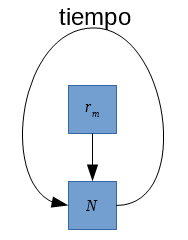
\includegraphics[width=.45\textwidth]{figuras/blockDiagrExpGrowth.png}\label{fig:diffGrowthModelsA}}
        \subfloat[Crecimiento logístico]{%
            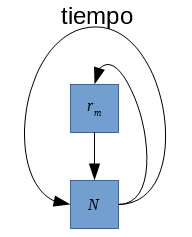
\includegraphics[width=.45\textwidth]{figuras/blockDiagrLogGrowth.png}\label{fig:diffGrowthModelsB}}
         \caption{Diferencias en los modelos de crecimiento}
        \label{fig:diffGrowthModels}
    \end{figure}

Independientemente de las razones que causen la disminución del
crecimiento, podemos entender que la tasa intrínseca de crecimiento
(\(r_m\)), en realidad no es una constante como en el modelo de
crecimiento exponencial (Figura \ref{fig:diffGrowthModelsA}); más bien,
es una función del tamaño de población, \(N\) (Figura
\ref{fig:diffGrowthModelsB}).

\[
r_m = f \left( N_t \right)
\]

Esta función debe tener algunas características particulares. Por
ejemplo, debe ser máxima cuando el tamaño de población es pequeño,
asumiendo que en ese momento hay muchos recursos y espacio para todos
los
individuos\footnote{Ignoramos el hecho de que en tamaños muy pequeños de población, existe problemas genéticos, o para encontrar pareja (Efecto Allee), que provocarían un crecimiento negativo.}.
Por otro lado, cuando la población alcanza un tamaño grande, la tasa de
crecimiento debe disminuir hasta llegar a cero.

Debemos introducir un nuevo término a nuestro modelo de crecimiento,
para cumplir con las características descritas arriba. Este término es
la \emph{capacidad de carga}, \(K\), que es el punto donde la tasa de
crecimiento se vuelve cero.

Una expresión que cumple con estos requerimientos es:

\[
 r_m = \mathrm{r_m}\left(1-\frac{N_t}{K}\right)
\]

Podemos observar el comportamiento de \(r_m\) con un gráfico:

\begin{Shaded}
\begin{Highlighting}[]
\NormalTok{rm <-}\StringTok{ }\DecValTok{1}
\NormalTok{K <-}\StringTok{ }\DecValTok{100}
\NormalTok{N <-}\StringTok{ }\DecValTok{0}\OperatorTok{:}\DecValTok{100}

\NormalTok{val <-}\StringTok{ }\NormalTok{rm }\OperatorTok{*}\StringTok{ }\NormalTok{(}\DecValTok{1} \OperatorTok{-}\StringTok{ }\NormalTok{(N }\OperatorTok{/}\StringTok{ }\NormalTok{K))}

\KeywordTok{plot}\NormalTok{(N,}
\NormalTok{  val,}
  \DataTypeTok{type =} \StringTok{"l"}\NormalTok{, }\DataTypeTok{las =} \DecValTok{1}\NormalTok{, }\DataTypeTok{lwd =} \DecValTok{2}\NormalTok{,}
  \DataTypeTok{xlab =} \StringTok{"Tamaño de población",}
\StringTok{  ylab = expression(r[m])}
\StringTok{  )}
\end{Highlighting}
\end{Shaded}

\begin{center}\includegraphics[width=0.7\linewidth]{dinPob_files/figure-latex/unnamed-chunk-2-1} \end{center}

Si ahora sustituimos la versión denso-dependiente de \(r_m\) en la
ecuación \eqref{eq:expG}, obtenemos

\begin{equation}
\frac{dN}{dt}=\mathrm{r_m} N_t \left(1-\frac{N_t}{K}\right)
 \label{eq:logi1}
\end{equation}

Esta ecuación diferencial también puede resolverse por el método de
separación de variables (ver Ejemplo \ref{exm:exp1}). Una vez resuelta,
la expresión en función del tiempo es:

\begin{equation}
N_t= \frac{K}{1+\left(\frac{K}{N_0}-1\right)e^{-rt}}
 \label{eq:logi2}
\end{equation}

Podemos graficar el comportamiento de la curva para una población
hipotética con: \(\mathrm{r_m} = 0.4\), \(K = 100\), y \(N_0 = 10\).
Para ello, usamos el siguiente código:

\begin{Shaded}
\begin{Highlighting}[]
\NormalTok{r <-}\StringTok{ }\FloatTok{0.4}
\NormalTok{K <-}\StringTok{ }\DecValTok{100}
\NormalTok{N0 <-}\StringTok{ }\DecValTok{10}
\KeywordTok{curve}\NormalTok{(}
\NormalTok{  K}\OperatorTok{/}\NormalTok{(}\DecValTok{1}\OperatorTok{+}\NormalTok{((K}\OperatorTok{/}\NormalTok{N0}\OperatorTok{-}\DecValTok{1}\NormalTok{)}\OperatorTok{*}\KeywordTok{exp}\NormalTok{(}\OperatorTok{-}\NormalTok{r}\OperatorTok{*}\NormalTok{x))),}
  \DataTypeTok{from =} \DecValTok{0}\NormalTok{,}\DataTypeTok{to =} \DecValTok{20}\NormalTok{,}
  \DataTypeTok{las =} \DecValTok{1}\NormalTok{, }\DataTypeTok{lwd =} \DecValTok{2}\NormalTok{, }
  \DataTypeTok{xlab =} \StringTok{"Tiempo"}\NormalTok{, }\DataTypeTok{ylab =} \StringTok{"Tamaño de Población")}
\end{Highlighting}
\end{Shaded}

\begin{figure}[h]

{\centering \includegraphics[width=0.7\linewidth]{dinPob_files/figure-latex/unnamed-chunk-3-1} 

}

\caption{Crecimiento logístico, con capacidad de carga igual a cien individuos}\label{fig:unnamed-chunk-3}
\end{figure}

Observamos que la población ya no crece de manera indefinida. Ahora
tiene un tope superior igual a la capacidad de carga, \(K\).
Técnicamente, decimos que existe un límite asintótico al crecimiento; ya
que, el tamaño de población \emph{tiende} a \(K\), pero nunca llega a
alcanzarlo (pero ver ejercicio \ref{exr:logGrowth2}).

Por otro lado, observamos que la población crece rápidamente al inicio;
pero, al final de la curva el crecimiento se detiene. Esto implica que
en algún punto, el crecimiento alcanza un máximo. Este punto se conoce
como el \emph{punto de inflexión}.

De cálculo diferencial, sabemos que los puntos de inflexión se obtienen
al igualar la segunda derivada de la función a cero:

\[
\frac{d^2N}{dt^2}=\frac{d(dN)}{d(dt)}=0
\]

Sabemos que la primer derivada de \(N_t\) corresponde a la ecuación
\eqref{eq:logi1}. Entonces, para encontrar el punto de inflexión, primero
debemos encontrar:

\[
\frac{d^2N}{dt^2}=\frac{d(dN)}{d(dt)}=D\left[ \mathrm{r_m}N_t\left(1-\frac{N_t}{K}\right)\right]=0
\]

Se utiliza la regla del producto, y se tiene:

\[
D_{N_t}\left[ \mathrm{r_m}N_t \right]\left(1-\frac{N_t}{K}\right) + \mathrm{r_m}N_t\; D_{N_t}\left[\left(1-\frac{N_t}{K}\right)\right]=0
\]

Al resolver las derivadas se obtiene:

\[
N = \frac{K}{2}
\]

Quiere decir, que el mayor crecimiento se obtiene cuando el tamaño de
población es igual a la mitad de la capacidad de carga. Si sustituimos
\(N = K/2\) en la ecuación \eqref{eq:logi1}, tenemos que el crecimiento
máximo de una población
es\footnote{La línea vertical a mano izquierda en la ecuación indica que la derivada debe evaluarse en $N_t=K/2$.}:

\[
\left. \frac{dN}{dt}\right|_{N = K/2} = \frac{\mathrm{r_m}K}{4}
\]

Esto tiene grandes implicaciones en el manejo de recursos naturales. Es
la base de los modelos de producción excedentaria. En pesquerías, a este
número se le conoce como \emph{Máximo Rendimiento Sostenible}; sin
embargo, ha sido fuertemente criticado \citep{Larkin1977}, y en la
actualidad se utilizan algunas variantes de esta cantidad, o otros
modelos más apropiados, basados en estructura de edades o tallas.

\subsection{Usos del modelo logístico}\label{usos-del-modelo-logistico}

En la sección anterior calculamos el \emph{Máximo Rendimiento
Sostenible} (MRS). Ahora lo definiremos como:

\begin{quote}
El crecimiento máxmimo que una población puede producir, bajo una
capacidad de carga determinada. Ésta es la cantidad máxima de
individuos, o biomasa, que se puede extraer de una población, sin
provocar un crecimiento negativo.
\end{quote}

Recordando que:

\begin{quote}
Tamaño de población = Tamaño anterior + Crecimiento
\end{quote}

La idea de \emph{cosechar} una población se fundamenta en que si se
extrae una cantidad igual al crecimiento de la población, la biomasa
restante logrará regenerarse y crecer. La idea del MRS, es que el tamaño
de una población cosechada, debe llevarse a \(N/2\), para poder
aprovechar el crecimiento máximo que puede generar dicha población.

\BeginKnitrBlock{exercise}
\protect\hypertarget{exr:logGrowth2}{}{\label{exr:logGrowth2} }Demuestre que
la población no crecerá más cuando llega a la capacidad de carga. Es
decir, tome el límite de la ecuación \eqref{eq:logi1}, cuando
\(t \to \infty\).
\EndKnitrBlock{exercise}

\BeginKnitrBlock{exercise}
\protect\hypertarget{exr:logGrowth3}{}{\label{exr:logGrowth3} }Suponga que
existe un tanque sobre una balanza. Este tanque contiene aguas
residuales, que son limpiadas por una pequeña planta del genero
\emph{Lemna}. El flujo del tanque es tal, que la masa del agua siempre
se mantiene constante; de modo que la balanza solo mide el crecimiento
de \emph{Lemna}. Nos interesa mantener una población de Lemna con un
rápido crecimiento; ya que éste es proporcional a la tasa de extracción
de toxinas del tanque. El tanque inicia con \SI{1}{\kilogram} de
\emph{Lemna}, con una tasa de crecimiento es de \SI{5e-6}{\per\second}.
Además, se ha determinado que el tanque solo soporta \SI{100}{\kilogram}
de \emph{Lemna}. ¿Cuál es el tamaño de población de \emph{Lemna} que
debería haber en el tanque para maximizar el crecimiento? ¿Cuánta
biomasa debe extraer \textbf{en un día} para mantener un máximo de
crecimiento? ¿A qué biomasa total debería cosechar la \emph{Lemna}?
\EndKnitrBlock{exercise}

\BeginKnitrBlock{exercise}
\protect\hypertarget{exr:logGrowth4}{}{\label{exr:logGrowth4} }De acuerdo
con la definición del MRS, se asume que el crecimiento es igual a la
cosecha. ¿Qué tan atinada es esta suposición?
\EndKnitrBlock{exercise}

\BeginKnitrBlock{exercise}
\protect\hypertarget{exr:logGrowth5}{}{\label{exr:logGrowth5} }Grafique la
tasa de crecimiento poblacional usando \(N_t\) como variable
independiente. Asuma \(K=100\), \(N_0=1\), \(r_m=1\).
\EndKnitrBlock{exercise}

\subsection{Matrices}\label{matrices}

\href{http://onlinelibrary.wiley.com/doi/10.1111/1365-2656.12482/full}{COMADRE}
\href{http://www.compadre-db.org/Data/Comadre}{COMADRE DATA} Ojo a la
guia de usuario

\section{Otras fuentes
bibliográficas}\label{otras-fuentes-bibliograficas}

Esta sección está basada en los capítulos 4 y 5 de \citet{NealPopBio}.
En la sección 2.3 de \citet{PopSystem}, se desarrollan los mismos
modelos básicos vistos aquí; en este mismo libro se presenta una buena
introducción sobre la ecología de poblaciones como \emph{sistemas}, en
el capítulo 1.

\chapter{Soluciones a los ejercicios}\label{soluciones-a-los-ejercicios}

\textbf{Ejercicio \ref{exr:plotGeomGrowth}}

\begin{Shaded}
\begin{Highlighting}[]
\KeywordTok{plot}\NormalTok{(}\DecValTok{0}\NormalTok{,}\DecValTok{0}\NormalTok{,}\DataTypeTok{xlim =} \KeywordTok{c}\NormalTok{(}\DecValTok{0}\NormalTok{,}\DecValTok{50}\NormalTok{),}
     \DataTypeTok{ylim =} \KeywordTok{c}\NormalTok{(}\DecValTok{0}\NormalTok{,}\DecValTok{100}\NormalTok{) ,}
     \DataTypeTok{type =} \StringTok{'n'}\NormalTok{,}\DataTypeTok{xlab =} \StringTok{'Tamaño poblacional'}\NormalTok{,}
     \DataTypeTok{ylab =} \StringTok{"Tasa de crecimiento"}\NormalTok{)}

\NormalTok{val=}\KeywordTok{numeric}\NormalTok{()}

\ControlFlowTok{for}\NormalTok{(Rm }\ControlFlowTok{in} \KeywordTok{c}\NormalTok{(}\OperatorTok{-}\DecValTok{1}\NormalTok{,}\DecValTok{0}\NormalTok{,}\DecValTok{1}\NormalTok{))\{}
  \KeywordTok{abline}\NormalTok{(}\DecValTok{50}\NormalTok{,Rm,}\DataTypeTok{lty=}\NormalTok{Rm}\OperatorTok{+}\DecValTok{2}\NormalTok{)}
\NormalTok{  val=}\KeywordTok{append}\NormalTok{(val,Rm)}
\NormalTok{\}}
\KeywordTok{legend}\NormalTok{(}\StringTok{"topleft"}\NormalTok{,}\DataTypeTok{lty=} \DecValTok{1}\OperatorTok{:}\DecValTok{3}\NormalTok{,}\DataTypeTok{legend =} \KeywordTok{paste}\NormalTok{(}\StringTok{'Rm = '}\NormalTok{,val))}
\end{Highlighting}
\end{Shaded}

\begin{center}\includegraphics[height=6cm]{dinPob_files/figure-latex/unnamed-chunk-4-1} \end{center}

\(R_m\) representa la pendiente de la recta.

\textbf{Ejercicio \ref{exr:GeomGrowthBacteria2}}

En 3 horas existen 12 periodos de 15 minutos (\(t=12\)). Entonces
aplicamos la ecuación \eqref{eq:geom2}:

\[
100\times 2^{12} = \num{409600}\text{ células}
\]

\textbf{Ejercicio \ref{exr:expGrowth1}}

Obtener \(r_m = \ln \lambda\); luego multiplicar
\(r_{mes}=r_m \times 4\) para obtener la escala a meses. Finalmente,
transformar \(\lambda_{mes}=e^{r_{mes}}\).

\textbf{Ejercicio \ref{exr:expGrowth3}}

Asumimos que \(r_m\) es cualquier constante positiva
(\(r_m \in \mathbb{R}^+\)). Entonces \(-1\times r_m \in \mathbb{R}^-\).

Luego, tomamos el límite:

\[
\lim_{t \to \infty}N_0 e^{-r_m t}
\]

Que equivale a:

\[
\lim_{t \to \infty}\frac{N_0}{e^{r_m t}}
\]

Vemos que el denominador de la expresión anterior es un número que
crecerá infinitamente. Si reemplazamos \(e^{r_m t}\) por \(x\), cuando
\(t \to \infty \Rightarrow x \to \infty\). Y quedamos con la expresión:

\[
\lim_{x \to \infty}\frac{N_0}{x} = 0
\]

Porque cuando \(x \to \infty \Rightarrow x \gg N_0\). Es decir, cuando
\(x\) se vuelve infinito, es mucho más grande que \(N_0\), por tanto, el
cociente tiende a cero, cuando \(x\) tiende a infinito.

Poblacionalmente, esto significa, que si una población mantiene una tasa
intrínseca negativa, por un periodo de tiempo suficientemente largo,
sufrirá un evento de extinción.

\textbf{Ejercicio \ref{exr:logGrowth3}}

\emph{El tamaño de población que maximiza el crecimiento}

Reconocemos que la capacidad de carga son \(K=\SI{100}{\kilogram}\). Por
tanto, la cantidad de biomasa que maximiza el crecimiento, según el
\emph{máximo rendimiento sostenible} es \(K/2=\SI{50}{\kilogram}\).

\emph{¿Cuánta biomasa se debe extraer en un día para mantener la tasa de
crecimiento al máximo?}

Debemos utilizar unidades congruentes durante los cálculos. Así que el
primer paso convertir \(r_m\) de \si{\per\second} a \si{\per\day}.

\[
\frac{\num{5e-6} }
{\cancel{ \si{\second} } }
\frac{\num{86400}\cancel{\si{\second}} }{\si{\day}}= 
\frac{\num{0.432}}
{\si{\day}}
\]

Ahora podemos calcular el \emph{Máximo Rendimiento Sostenible},
reemplazando los valores apropiados en:

\[
MRS=\frac{r_m K}{4} = \SI{10.8}{\kilogram}
\]

\emph{¿A qué biomasa total se debe cosechar el tanque?}

Esta es la suma del tamaño de población al \emph{máximo rendimiento
sostenible}, más el \emph{máximo rendimiento sostenible}:

\[
\frac{K}{2} + \frac{r_m K}{4} = \SI{60.8}{\kilogram}
\]

\begingroup
\small
\printindex
\vfill
\endgroup

\appendix


\chapter{Métodos numéricos para ecología de
poblaciones}\label{metodos-numericos-para-ecologia-de-poblaciones}

\section{Simulación de ecuaciones
diferenciales}\label{simulacion-de-ecuaciones-diferenciales}

Tomaremos el ejemplo de la ecuación \eqref{eq:diffG}, para mostrar un
método para encontrar el tamaño de población, sin tener que utilizar
cálculo \citep{Barrantes2015}. Este es el \emph{método de Euler}, que se
explicará mediante un ejemplo.

Una derivada implica un cambio infinitesimal de una variable en relación
a otra. Por ejemplo, el cambio en el número de individuos de una
población en un momento pequeñísimo de tiempo, puede representarse como
la diferencia de la población, entre la duración de ese pequeño
intervalo de tiempo:

\[
\frac{dN}{dt} \approx \frac{\Delta N}{\Delta t} = \frac{N_t - N_{t-\Delta t}}{\Delta t}
\]

Si sustituimos en la ecuación \eqref{eq:expG}, tenemos:

\[
\frac{N_t - N_{t-\Delta t}}{\Delta t} = r_m N
\]

Arreglando la expresión anterior, podemos despejar en terminos de
\(N_t\):

\[
N_t= N_{t-\Delta t} + r_m N_{t-\Delta t} \Delta t
\]

Hay que resaltar que esta \textbf{no} es una solución exacta; sino, una
aproximación. Entre más pequeño se haga \(\Delta t\), más se aproximará
el resultado, al valor exacto dado por \eqref{eq:expG}. En casos donde no
existe una solución analítica, o simplemente, no es sencillo resolver la
ecuación, siempre se puede recurrir a los métodos numéricos, para tener
una idea de la solución real.

Para programar este sencillo ejemplo, necesitamos varios pasos:

\begin{itemize}
\item
  Definir un valor inicial de la población, y el valor de \(t\) en el
  cuál queremos conocer el tamaño de población.
\item
  Definir el Valor de \(r_m\).
\item
  Establecer un criterio para guardar el valor de \(N_t\), cada cierto
  lapso de tiempo. (Para no crear un objeto virtual innecesariamente
  grande)
\item
  Crear un objeto para guardar el tamaño de la población, y los puntos
  de tiempo a los que está asociada.
\item
  Definir el tamaño de \(\Delta t\), y calcular el número de iteraciones
  necesarias hasta llegar al final del periodo de tiempo de interés.
\item
  Crear un bucle, y ejecutar iteractivamente la integración de Euler.
\item
  Definir un criterio para detener el algoritmo.
\end{itemize}

El siguiente algoritmo generaliza todas las funciones dependientes de
\(N_{t-\Delta t}\).

\[
N_t= N_{t-\Delta t} + f \left( N_{t-\Delta t},\mathbf{c} \right) \Delta t
\]

Donde \(\mathbf{c}\) son constantes.

\begin{Shaded}
\begin{Highlighting}[]
\NormalTok{euler <-}\StringTok{ }\ControlFlowTok{function}\NormalTok{(fooName, valInic, tiempoParar, deltaT,guardarCada,...)\{}
\NormalTok{  arg <-}\StringTok{ }\KeywordTok{list}\NormalTok{(...)}
\NormalTok{  fn <-}\StringTok{ }\KeywordTok{get}\NormalTok{(fooName)}
  
  \CommentTok{#Encuentra los argumentos provistos}
\NormalTok{  argName <-}\StringTok{ }\KeywordTok{match.arg}\NormalTok{(}\KeywordTok{names}\NormalTok{(arg),}\CommentTok{#arg provistos}
                       \KeywordTok{formalArgs}\NormalTok{(fn),}\CommentTok{#arg existentes}
                       \DataTypeTok{several.ok =} \OtherTok{TRUE}\NormalTok{)}
  \CommentTok{#Nombra la lista con los nombres de los argumentos provistos}
  \KeywordTok{names}\NormalTok{(arg) <-}\StringTok{ }\NormalTok{argName}
  
\NormalTok{  val <-}\StringTok{ }\KeywordTok{numeric}\NormalTok{()}
\NormalTok{  val[}\DecValTok{1}\NormalTok{] <-}\StringTok{ }\NormalTok{valInic}
  
\NormalTok{  valTmp <-}\StringTok{ }\KeywordTok{numeric}\NormalTok{()}
\NormalTok{  valTmp <-}\StringTok{ }\NormalTok{val[}\DecValTok{1}\NormalTok{]}
  
  \CommentTok{#Completa la lista de argumentos con N[t-1]}
\NormalTok{  arg[[ (}\KeywordTok{length}\NormalTok{(arg)}\OperatorTok{+}\DecValTok{1}\NormalTok{) ]] <-}\StringTok{ }\NormalTok{valInic}
\NormalTok{  totalArg <-}\StringTok{ }\KeywordTok{length}\NormalTok{(arg)}
  \CommentTok{#Escribe todos los nomres de los argumentos, para do.call}
  \KeywordTok{names}\NormalTok{(arg) <-}\StringTok{ }\KeywordTok{formalArgs}\NormalTok{(fn)}\CommentTok{#Encuetra los nombres de los argumentos}
  
\NormalTok{  tiempo <-}\StringTok{ }\KeywordTok{numeric}\NormalTok{()}
  
\NormalTok{  tNow <-}\StringTok{ }\DecValTok{0}
\NormalTok{  tiempo[}\DecValTok{1}\NormalTok{] <-}\StringTok{ }\DecValTok{0}
  
  \ControlFlowTok{while}\NormalTok{( tNow }\OperatorTok{<}\StringTok{ }\NormalTok{tiempoParar )\{}
\NormalTok{    valTmp <-}\StringTok{ }\NormalTok{valTmp }\OperatorTok{+}\StringTok{ }\KeywordTok{do.call}\NormalTok{(fn,}\DataTypeTok{args =}\NormalTok{ arg)}\OperatorTok{*}\NormalTok{deltaT}
\NormalTok{    tNow <-}\StringTok{ }\NormalTok{tNow }\OperatorTok{+}\StringTok{ }\NormalTok{deltaT }
      
    \ControlFlowTok{if}\NormalTok{( tNow}\OperatorTok\NormalTok{guardarCada }\OperatorTok{<=}\NormalTok{deltaT )\{}
\NormalTok{      val <-}\StringTok{ }\KeywordTok{append}\NormalTok{(}\DataTypeTok{x =}\NormalTok{ val,}\DataTypeTok{values =}\NormalTok{ valTmp)}
\NormalTok{      tiempo <-}\StringTok{ }\KeywordTok{append}\NormalTok{(}\DataTypeTok{x =}\NormalTok{ tiempo, }\DataTypeTok{values =}\NormalTok{ tNow)}
\NormalTok{      arg[[totalArg]] <-}\StringTok{ }\NormalTok{valTmp}
\NormalTok{    \}}
\NormalTok{  \}}
  
  \KeywordTok{return}\NormalTok{( }\KeywordTok{list}\NormalTok{(}
    \DataTypeTok{poblacion =}\NormalTok{ val,}
    \DataTypeTok{tiempo =}\NormalTok{ tiempo,}
    \DataTypeTok{tNow =}\NormalTok{ tNow,}
    \DataTypeTok{arg =}\NormalTok{ arg}
\NormalTok{  ) )}
  
\NormalTok{\}}
\end{Highlighting}
\end{Shaded}

Por ejemplo

\begin{Shaded}
\begin{Highlighting}[]
\NormalTok{diffG1 <-}\StringTok{ }\ControlFlowTok{function}\NormalTok{(rm, N) N }\OperatorTok{*}\StringTok{ }\NormalTok{rm}
\NormalTok{N0 <-}\StringTok{ }\DecValTok{10}

\NormalTok{Resultados1 <-}\StringTok{ }\KeywordTok{euler}\NormalTok{(}\DataTypeTok{fooName =} \StringTok{"diffG1"}\NormalTok{, }\DataTypeTok{valInic =}\NormalTok{ N0, }\DataTypeTok{tiempoParar =} \DecValTok{10}\NormalTok{, }\DataTypeTok{deltaT =} \DecValTok{1}\OperatorTok{/}\DecValTok{100}\NormalTok{, }
    \DataTypeTok{guardarCada =} \DecValTok{1}\NormalTok{, }\DataTypeTok{rm =} \FloatTok{0.22}\NormalTok{)}

\NormalTok{diffG2 <-}\StringTok{ }\ControlFlowTok{function}\NormalTok{(rm, Kmax, N) rm }\OperatorTok{*}\StringTok{ }\NormalTok{(}\DecValTok{1} \OperatorTok{-}\StringTok{ }\NormalTok{N}\OperatorTok{/}\NormalTok{Kmax)}

\NormalTok{N0 <-}\StringTok{ }\DecValTok{10}

\NormalTok{Resultados2 <-}\StringTok{ }\KeywordTok{euler}\NormalTok{(}\DataTypeTok{fooName =} \StringTok{"diffG2"}\NormalTok{, }\DataTypeTok{valInic =}\NormalTok{ N0, }\DataTypeTok{tiempoParar =} \DecValTok{50}\NormalTok{, }\DataTypeTok{deltaT =} \DecValTok{1}\OperatorTok{/}\DecValTok{100}\NormalTok{, }
    \DataTypeTok{guardarCada =} \DecValTok{1}\NormalTok{, }\DataTypeTok{rm =} \FloatTok{1.92}\NormalTok{, }\DataTypeTok{Kmax =} \DecValTok{60}\NormalTok{)}

\KeywordTok{plot}\NormalTok{(Resultados1}\OperatorTok{$}\NormalTok{tiempo, Resultados1}\OperatorTok{$}\NormalTok{poblacion, }\DataTypeTok{type =} \StringTok{"p"}\NormalTok{, }\DataTypeTok{xlab =} \StringTok{"Tiempo"}\NormalTok{, }
    \DataTypeTok{ylab =} \StringTok{"Tamaño de población", las = 1, pch = 21, bg = 1)}
\StringTok{lines(Resultados1$tiempo, Resultados1$poblacion)}
\end{Highlighting}
\end{Shaded}

\includegraphics{dinPob_files/figure-latex/unnamed-chunk-7-1.pdf}

\begin{Shaded}
\begin{Highlighting}[]
\KeywordTok{plot}\NormalTok{(Resultados2}\OperatorTok{$}\NormalTok{tiempo, Resultados2}\OperatorTok{$}\NormalTok{poblacion, }\DataTypeTok{type =} \StringTok{"p"}\NormalTok{, }\DataTypeTok{xlab =} \StringTok{"Tiempo"}\NormalTok{, }
    \DataTypeTok{ylab =} \StringTok{"Tamaño de población", las = 1, pch = 21, bg = 1)}
\StringTok{lines(Resultados2$tiempo, Resultados2$poblacion)}
\end{Highlighting}
\end{Shaded}

\includegraphics{dinPob_files/figure-latex/unnamed-chunk-7-2.pdf}

\chapter{Tutorial de R con RStudio}\label{tutorial-de-r-con-rstudio}

\section{\texorpdfstring{Crear un proyecto en
\emph{RStudio}}{Crear un proyecto en RStudio}}\label{RStudioProject}

Crear un proyecto en \textbf{RStudio} para cualquier proyecto con
\textbf{R}, es importante. Los proyectos organizan los documentos en una
sola carpeta, y son fundamentales para el control de versión con un
software como \textbf{Git}.

Abrimos \textbf{RStudio}, y ubicamos la barra de herramientas en la
parte superior. El primer paso es ir a
\texttt{file\ -\/-\textgreater{}\ New\ Project}. Creamos una carpeta en
una ubicación que nos permita tener derechos de administrador, e
idealmente, fuera de cualquier carpeta de sincronización en
línea\footnote{En caso de que quieran tener un respaldo en la nube, se recomienda pausar la sincronización mientras se trabaja en el proyecto}.

RStudio nos guiará por los siguientes pasos:

\begin{itemize}
\item
  \texttt{Crear\ un\ Proyecto}: Escogemos que sea un nuevo directorio.
\item
  \texttt{Tipo\ de\ Proyecto}: Escogemos \emph{nuevo proyecto}.
\item
  \texttt{Crear}: Escogemos la carpeta, y el nombre del proyecto.
  \textbf{NO} marcamos \emph{crear repositorio con Git}.
\end{itemize}

\begin{figure}[thb!]

{\centering 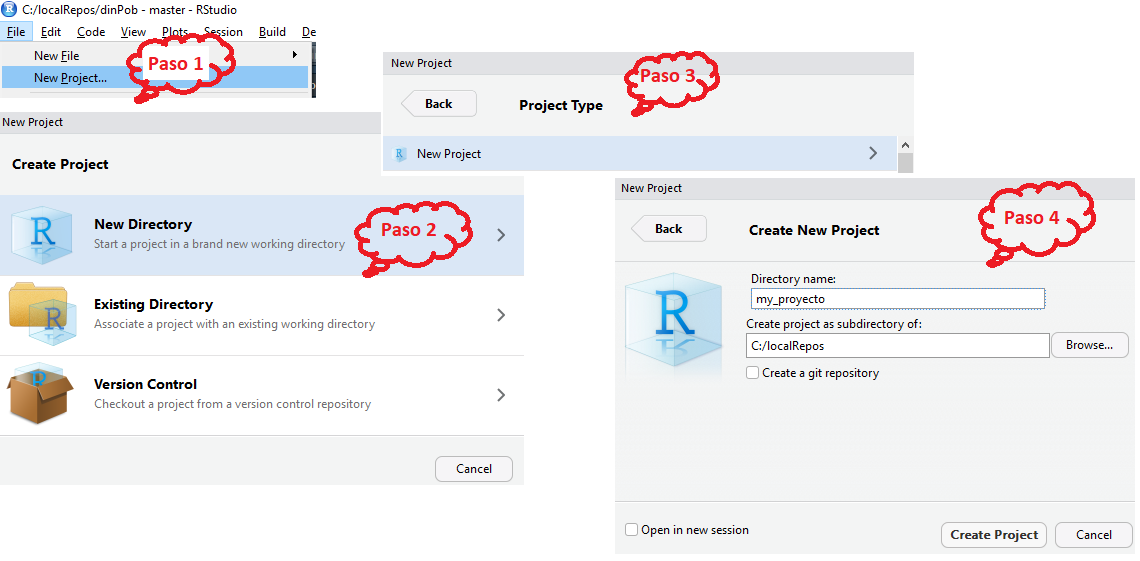
\includegraphics[width=0.95\linewidth]{figuras/RStudioNewProject} 

}

\caption{Cómo hacer un nuevo proyecto, en \textbf{RStudio}.}\label{fig:RStudioNewProject}
\end{figure}

Volvemos a la barra de herramientas, en \textbf{RStudio}, y vamos a
\texttt{File\ -\/-\textgreater{}\ New\ file\ -\/-\textgreater{}\ R\ script}.
Este archivo solo soporta código en \textbf{R}, con la gran ventaja de
que colorea las funciones, variables y estructuras más comunes; lo cual,
hace que el código sea más legible.

\textbf{IMPORTANTE}: En el siguiente tutorial, el código en \textbf{R}
se encuentra dentro de ambientes especiales, rodeados por una caja gris.
Escribe las líneas que se muestran en esa caja, y para ver el resultado
en la consola de \textbf{R}, apreta \texttt{Ctrl\ +\ ENTER}.

\section{Funciones básicas en R}\label{funciones-basicas-en-r}

Ahora que hemos creado un proyecto, y tenemos un lienzo en blanco,
empezamos por ver las funciones más elementales. \textbf{R} contiene
todas las operaciones básicas como: adición, substracción,
multipliación, división, potencias, y logaritmos.

\begin{Shaded}
\begin{Highlighting}[]
\CommentTok{# Tras cada línea presiona Ctrl + ENTER}

\DecValTok{1} \OperatorTok{+}\StringTok{ }\DecValTok{1} \CommentTok{# adición}

\DecValTok{1}\OperatorTok{-}\DecValTok{1} \CommentTok{# substracción}

\DecValTok{1}\OperatorTok{*}\DecValTok{2} \CommentTok{# multiplicación}

\DecValTok{1}\OperatorTok{/}\DecValTok{2} \CommentTok{# división}

\DecValTok{2}\OperatorTok{^}\NormalTok{(}\DecValTok{8}\NormalTok{) }\CommentTok{#potencia}

\KeywordTok{log}\NormalTok{(}\DecValTok{2}\NormalTok{) }\CommentTok{# logaritmo natural}

\KeywordTok{log10}\NormalTok{(}\DecValTok{2}\NormalTok{) }\CommentTok{#logaritmo base 10}

\KeywordTok{log}\NormalTok{(}\DataTypeTok{x =} \DecValTok{2}\NormalTok{, }\DataTypeTok{base =} \OperatorTok{<}\NormalTok{n}\OperatorTok{>}\NormalTok{) }\CommentTok{#logaritmo base <n>, donde <n> se}
                       \CommentTok{#   reemplaza por cualquier número.}
\end{Highlighting}
\end{Shaded}

Notar que en el código, cualquier línea de texto precedida de
\texttt{\#} es un comentario, que no será evaluado por el computador.
Agregar comentarios es muy útil, si uno va a re-utilizar parte del
código en otro momento. Ayuda a mantener la claridad en lo que se está
haciendo.

Continuando con las operaciones básicas, también podemos mezclar
operaciones de la forma que convenga. Siempre considerando las reglas de
prioridad por paréntesis. Por ejemplo, si queremos calcular el logaritmo
del resultado de una función, para una base 16.

\begin{Shaded}
\begin{Highlighting}[]
\KeywordTok{log}\NormalTok{( }\DataTypeTok{x=} \DecValTok{1} \OperatorTok{/}\StringTok{ }\NormalTok{(}\DecValTok{1} \OperatorTok{+}\StringTok{ }\NormalTok{(}\DecValTok{5}\OperatorTok{/}\DecValTok{2}\NormalTok{) ) , }\DataTypeTok{base =} \DecValTok{16}\NormalTok{ )}
\end{Highlighting}
\end{Shaded}

Luego, como la mayoría de lenguajes de programación, podemos asignar
valores a un objeto y utilizarlo después en otra operación:

\begin{Shaded}
\begin{Highlighting}[]
\NormalTok{a <-}\StringTok{ }\KeywordTok{log10}\NormalTok{(}\DecValTok{4}\OperatorTok{/}\DecValTok{3}\NormalTok{)  }\CommentTok{# 'a' tiene el valor de la operación}

\NormalTok{b <-}\StringTok{ }\NormalTok{a}\OperatorTok{^}\DecValTok{2} \CommentTok{# Equivale a log10(4/3)^2}

\NormalTok{c <-}\StringTok{ }\NormalTok{b}\OperatorTok{^}\DecValTok{2} \OperatorTok{-}\StringTok{ }\NormalTok{a}

\NormalTok{c}
\end{Highlighting}
\end{Shaded}

Esto quiere decir que podemos crear un objeto con el operador
\texttt{\textless{}-}, que pueden ser datos, o resultados de otras
operaciones, para incluirlo en una nueva función. Por lo que la salida
de una función puede ser la entrada de la próxima.

\begin{figure}[thb!]

{\centering 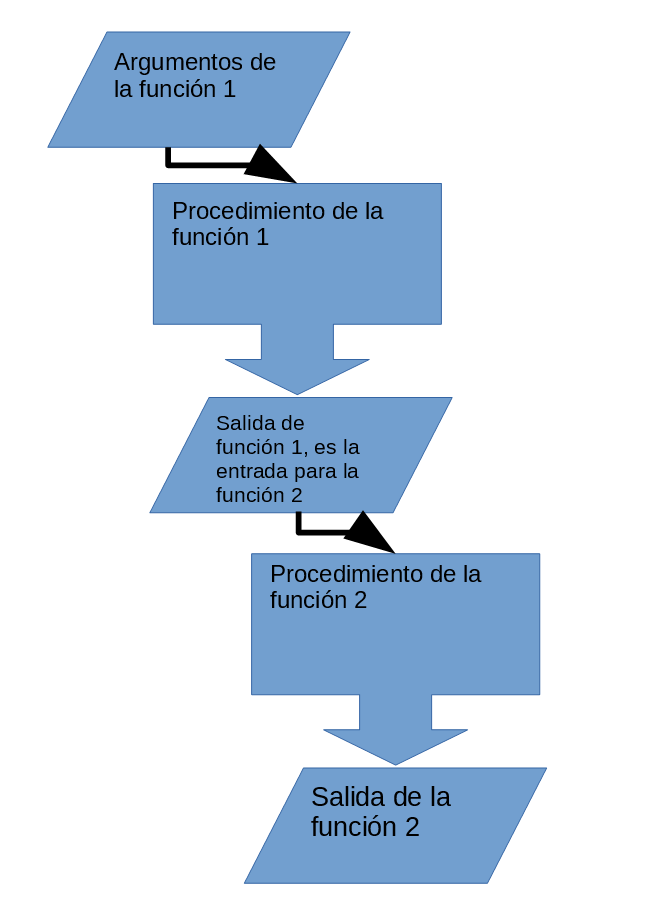
\includegraphics[width=0.4\linewidth]{figuras/RFunctionsFlow} 

}

\caption{Flujo de entradas y salidas en una función de \textbf{R}}\label{fig:RFunctionFlow}
\end{figure}

\section{Estructuras de datos}\label{estructuras-de-datos}

\textbf{R} puede manejar objetos muy complejos; sin embargo, estos
objetos generalmente se componen de partes muy sencillas. Revisaremos
éstas partes sencillas, y luego crearemos un objeto más complejo.

\textbf{Vectores}

Un vector en programación, es una colección de uno o más valores.
Podemos pensar que un vector en \textbf{R} equivale a una matriz de
\(n\) filas, y solo una columna.

\begin{Shaded}
\begin{Highlighting}[]
\NormalTok{vect1 <-}\StringTok{ }\KeywordTok{c}\NormalTok{(}\DecValTok{1}\NormalTok{,}\DecValTok{2}\NormalTok{,}\DecValTok{3}\NormalTok{,}\DecValTok{4}\NormalTok{,}\DecValTok{5}\NormalTok{,}\DecValTok{6}\NormalTok{,}\DecValTok{7}\NormalTok{,}\DecValTok{8}\NormalTok{,}\DecValTok{9}\NormalTok{,}\DecValTok{0}\NormalTok{) }\CommentTok{#es una concatenación de}
\CommentTok{# números, que se crea con la función 'c(...)'}

\NormalTok{vect2 <-}\StringTok{ }\KeywordTok{rnorm}\NormalTok{(}\DecValTok{10}\NormalTok{) }\CommentTok{# son diez números al azar obtenidas}
\CommentTok{# de una distribución normal estándar}
\end{Highlighting}
\end{Shaded}

Los elementos de un vector pueden ser llamados utilizando un sub-índice.
Éste inicia en 1, hasta \(n\). Donde \(n\) es la cantidad de elementos
en un vector.

\begin{Shaded}
\begin{Highlighting}[]
\NormalTok{vect1[}\DecValTok{3}\NormalTok{]}
\end{Highlighting}
\end{Shaded}

También es posible llamar varios elementos a la vez, si el subíndice del
vector es otro vector.

\begin{Shaded}
\begin{Highlighting}[]
\NormalTok{vect1[}\KeywordTok{c}\NormalTok{(}\DecValTok{3}\NormalTok{,}\DecValTok{4}\NormalTok{,}\DecValTok{5}\NormalTok{)]}

\NormalTok{vect1[}\DecValTok{3}\OperatorTok{:}\DecValTok{5}\NormalTok{] }
\CommentTok{# 3:5 crea una secuencia de enteros, que incrementa en 1 a la vez.}

\NormalTok{vect1[}\KeywordTok{rep}\NormalTok{(}\DecValTok{5}\NormalTok{,}\DataTypeTok{times=}\DecValTok{10}\NormalTok{)] }\CommentTok{# rep, es una función que repite un}
\CommentTok{#número un determinado número de veces.}
\end{Highlighting}
\end{Shaded}

Los vectores pueden ser datos en un archivo externo, o resultado de
funciones u operaciones. A diferencia de otros lenguajes \textbf{R},
maneja vectores de una forma más intuitiva.

\begin{Shaded}
\begin{Highlighting}[]
\NormalTok{vec3 <-}\StringTok{ }\NormalTok{vec1 }\OperatorTok{+}\StringTok{ }\NormalTok{vec2 }\CommentTok{# es un nuevo vector basado en la adición de los dos primeros.}
\end{Highlighting}
\end{Shaded}

\textbf{Matrices}

Las matrices son un arreglo de datos en dos dimensiones, es decir, filas
y columnas. Por covención, cuando decimos que una matriz es de tamaño
\(f\times c\), nos referimos a que tiene \(f\) filas, y \(c\) columnas.
Las filas siempre se nombran primero que las columnas.

\begin{Shaded}
\begin{Highlighting}[]
\NormalTok{(m1 <-}\StringTok{ }\KeywordTok{matrix}\NormalTok{(}\DecValTok{1}\OperatorTok{:}\DecValTok{9}\NormalTok{, }\DataTypeTok{ncol=}\DecValTok{3}\NormalTok{, }\DataTypeTok{byrow =}\NormalTok{ T) )}

\NormalTok{(m2 <-}\StringTok{ }\KeywordTok{matrix}\NormalTok{(}\DecValTok{1}\OperatorTok{:}\DecValTok{9}\NormalTok{, }\DataTypeTok{ncol=}\DecValTok{3}\NormalTok{, }\DataTypeTok{byrow =}\NormalTok{ F) )}
\end{Highlighting}
\end{Shaded}

Los elementos de una matriz se llaman por la combinación de filas y
columnas a la que corresponde. Del ejemplo anterior, si quisiéramos
obtener el elemento central de la matriz \texttt{m1}, lo llamamos así
\texttt{m1{[}2,2{]}}.

Si quisiéramos llamar toda la primer columna, entonces escribimos
\texttt{m1{[},1{]}}. O la primer y tercer fila \texttt{m1{[}c(1,3),{]}}.

Las operaciones con matrices suelen ser más delicadas y existen
operadores específicos para ellas.

\textbf{Marco de datos} o \emph{Data frames}

Esta estructura es similar a una matriz, con la diferencia, que algunas
de sus columnas pueden contener \emph{factores}, y no solo valores
numéricos. Estas son las estructuras con las que representamos un diseño
experimental, por ejemplo:

\begin{verbatim}
##   Var1 Var2          z
## 1   T1    a -0.2812197
## 2   T2    a  0.6062620
## 3   T1    b  0.9152684
## 4   T2    b  0.4222688
## 5   T1    c  0.4424541
## 6   T2    c -2.9359156
\end{verbatim}

\textbf{Arreglos} o \emph{arrays}

Estos son matrices de 3 o más dimensiones. Por ejemplo, si tenemos una
serie de fotografías con la misma resolución, en el mismo lugar, podemos
representar los pixeles como una matriz \(f\times c\), y el tiempo como
una dimensión adicional. Si ponemos en rápida sucesión las matrices,
tendremos un video o película.

\begin{Shaded}
\begin{Highlighting}[]
\KeywordTok{array}\NormalTok{(}\DecValTok{1}\OperatorTok{:}\NormalTok{(}\DecValTok{6}\OperatorTok{*}\DecValTok{2}\NormalTok{),}\DataTypeTok{dim=}\NormalTok{(}\KeywordTok{c}\NormalTok{(}\DecValTok{2}\NormalTok{,}\DecValTok{3}\NormalTok{,}\DecValTok{2}\NormalTok{)))}
\end{Highlighting}
\end{Shaded}

\textbf{Listas}

Las listas son colecciones de cualquiera de los objetos anteriores (y
otros que no hemos visto).

\begin{Shaded}
\begin{Highlighting}[]
\NormalTok{l1 <-}\StringTok{ }\KeywordTok{list}\NormalTok{(}
  \DataTypeTok{vector =}\NormalTok{ vect1,}
  \DataTypeTok{matriz =}\NormalTok{ m1}
  
\NormalTok{)}
\end{Highlighting}
\end{Shaded}

Podemos llamar a los elementos de una lista, de dos formas: si conocemos
el orden de los elementos de la lista, entonces, escribimos el índice
dentro de dos pares de corchetes rectos: \texttt{l1{[}{[}1{]}{]}}, para
llamar el vector y \texttt{l1{[}{[}2{]}{]}}, para llamar la matriz. Si
conocemos los nombres de los elementos de la lista, usamos la siguiente
forma: \texttt{l1\$vector}, para el vector; y \texttt{l1\$matriz}, para
la matriz.

Una vez dentro del objeto de la lista, podemos llamar sus elementos de
manera tradicional. Por ejemplo, \texttt{l1\$matriz{[}2,2{]}}, para
llamar el elemento central de la matriz \emph{dentro de la lista}.

\section{Funciones}\label{funciones}

Las funciones se representan por un nombre, seguido de un paréntesis
redondo. Todo lo que esté dentro de ese paréntesis son sus argumentos.
Para finalizar la función, cerramos con un paréntesis redondo derecho:

\begin{Shaded}
\begin{Highlighting}[]
\KeywordTok{funcion}\NormalTok{(}\DataTypeTok{argumento1 =}\NormalTok{ valor1,  }\DataTypeTok{argumento2 =}\NormalTok{ valor }\DecValTok{2}\NormalTok{)}
\end{Highlighting}
\end{Shaded}

Nosotros podemos crear nuestras propias funciones en R. El procedimiento
es sencillo:

\begin{enumerate}
\def\labelenumi{\arabic{enumi}.}
\item
  Llamamos a la función con un nombre, y declaramos que se trata de una
  función
\item
  Nombramos los argumentos de la función. Podemos asignar valores por
  defecto. Los argumentos deben ir entre paréntesis redondos.
\item
  Escribimos el cuerpo de la función entre paréntesis tipo llave
  \texttt{\{\}}. El cuerpo de la función debe terminar con \emph{un
  solo} objeto que será retornado como salida del proceso.
\end{enumerate}

Por ejemplo, si queremos hacer nuestra propia función para calcular un
promedio. Primero debemos entender la fórmula subyacente:

\[
\bar{x}= \frac{1}{n} \sum_{i=1}^{n} X_i
\]

Es decir, sumamos todos los elementos de un vector de valores, y lo
dividimos por el
\emph{tamaño}\footnote{El tamaño del vector, se refiere al total de elementos que lo conforman}
del vector. Entonces, nuestro argumento será un vector, y nuestra
salida, un valor único con el promedio.

\begin{Shaded}
\begin{Highlighting}[]
\NormalTok{promedio <-}\StringTok{ }\ControlFlowTok{function}\NormalTok{(vectorX)\{}
 
\NormalTok{   sumaX <-}\StringTok{ }\KeywordTok{sum}\NormalTok{(vectorX)}
   
\NormalTok{  n <-}\StringTok{ }\KeywordTok{length}\NormalTok{(vectorX) }\CommentTok{#length(), es una función que calcula }
                       \CommentTok{#   el tamaño del vector.}
\NormalTok{  valor <-}\StringTok{ }\NormalTok{sumaX }\OperatorTok{/}\StringTok{ }\NormalTok{n }
  
  \KeywordTok{return}\NormalTok{(valor)}
  
\NormalTok{\}}

\CommentTok{# Ahora probamos la función, tomando el promedio de un }
\CommentTok{#       vector de números normales con media igual a cero}
\CommentTok{#       Esperamos, que nuestro promedio sea un valor cercano}
\CommentTok{#         a cero.}

\NormalTok{valores <-}\StringTok{ }\KeywordTok{rnorm}\NormalTok{(}\DecValTok{100}\NormalTok{)}

\NormalTok{(}\KeywordTok{promedio}\NormalTok{(valores))}
\end{Highlighting}
\end{Shaded}

\begin{verbatim}
## [1] 0.07909427
\end{verbatim}

\chapter{Asignaciones}\label{asignaciones}

\section{\texorpdfstring{Tarea 01: ¡Hola mundo con
\emph{Rmarkdown}!}{Tarea 01: ¡Hola mundo con Rmarkdown!}}\label{tarea-01-hola-mundo-con-rmarkdown}

\textbf{Objetivo}: Verificar que el estudiante ha instalado, y maneja el
ambiente de trabajo que se utilizará durante el curso.

Primero revisa los enlaces provistos en el
\href{https://github.com/dawidh15/dinPob/wiki/02-Instalaci\%C3\%B3n-del-software-necesario\#prueba-con-rmarkdown}{wiki}.

\textbf{Actividades}

\begin{itemize}
\item
  Haz un nuevo proyecto en \textbf{RStudio}, que se llame
  \emph{Tarea01}. Ver pasos en sección \ref{RStudioProject}.
\item
  En la consola de \textbf{R}, escribe
  \texttt{install.packages(rmarkdown)}, con todas las dependencias. O
  instala el paquete desde \textbf{RStudio} como se mostró en el
  \href{https://github.com/dawidh15/dinPob/wiki/02-Instalaci\%C3\%B3n-del-software-necesario}{wiki}.
\item
  En \textbf{RStudio}
  \texttt{File-\/-\textgreater{}\ New\ File\ -\/-\textgreater{}\ R\ Markdown}.
\item
  Crea una sección principal que se llame \emph{Información
  profesional}.
\item
  Luego, crea una sección secundaria que se llame \emph{Intereses}. Usa
  bullets para nombrar algunos intereses profesionales.
\item
  Luego, crea una sección secundaria llamada \emph{Experiencia Laboral},
  si aplica. Nombra algunos trabajos relacionados con el curso de
  Ecología de Poblaciones.
\item
  Crea una sección principal que se llame \emph{Integración con R}
\item
  Consigue algunos datos interesantes en internet. Deben ser datos para
  graficar, por tanto deben tener dos columnas, y varias filas. Puedes
  ir a \href{https://www.wolframalpha.com/}{Wolfram Alpha}. Guarda los
  datos como un texto delimitado por comas (\texttt{.csv}).
\item
  En \textbf{R} o \textbf{RStudio} corre el comando
  \texttt{?read.table}. Para correr un comando en \textbf{RStudio}
  apreta \texttt{Cntrl\ +\ R}.
\item
  Crea un ``\emph{chunk}'' de código. Esto se hace en \textbf{RStudio},
  busca un botón en la barra especial de \emph{rmarkdown} que diga
  \texttt{insert}, luego escoge \texttt{R}.
\item
  Lee la tabla y asignala a un objeto:
\end{itemize}

\begin{Shaded}
\begin{Highlighting}[]
\NormalTok{datos <-}\StringTok{ }\KeywordTok{read.table}\NormalTok{(}\OperatorTok{<}\NormalTok{ruta_de_archivo_en_comillas}\OperatorTok{>}\NormalTok{,}
                    \DataTypeTok{header =} \OtherTok{TRUE}\NormalTok{,}
                    \DataTypeTok{sep =} \StringTok{","}\NormalTok{)}
\end{Highlighting}
\end{Shaded}

\begin{itemize}
\item
  Grafica los datos en un nuevo ``\emph{chunk}''. Usa el método que
  prefieras. Hay mucho material de cómo hacer gráficos en R. Por ahora,
  un gráfico básico es suficiente.
\item
  Ahora, haz otra sección llamada \emph{Bibliografía}. En un párrafo
  escribe una mini-revisión de algún tema que domines y del que
  dispongas referencias bibliográficas. Usa los mecanismos de citas de
  \emph{rmarkdown}

  \begin{itemize}
  \item
    Cita en texto con \texttt{@citationKey}
  \item
    Cita en paréntesis con \texttt{{[}@citationKey{]}}
  \end{itemize}
\end{itemize}

\begin{center}\rule{0.5\linewidth}{\linethickness}\end{center}

\textbf{Importante}: Para que las citas funcionen, debes agregar unas
opciones en la \emph{cabecera} del documento (\emph{YAML header}):

\begin{verbatim}
bibliography: <tu_archivo_bib>.bib
csl: apa.csl
\end{verbatim}

El archivo \texttt{apa.csl} se puede encontrar en google. Es un archivo
de estilo APA, para dar formato a la bibliografía. Revisa
\href{https://www.zotero.org/styles}{el repositorio de CSL de Zotero},
en busca de las revistas disponibles.

\begin{center}\rule{0.5\linewidth}{\linethickness}\end{center}

\begin{itemize}
\tightlist
\item
  Por último, corre el documento con el botón \texttt{knit}. Envía el
  documento \texttt{.Rmd} y el \texttt{.pdf} al profesor
  (\texttt{dawidh15@gmail.com}).
\end{itemize}

\newpage

\section{Tarea 02: Ejercicios de
crecimiento}\label{tarea-02-ejercicios-de-crecimiento}

Se recomienda hacer primero todo en papel, y luego pasarlo en limpio
usando \emph{Rmarkdown}. Uno de los aspectos más sobresalientes de LaTeX
es el aspecto de las ecuaciones. Los cálculos realizados en este
ejercicio son una buena excusa para investigar un poco sobre el tema. Se
recomienda este
\href{https://en.wikibooks.org/wiki/LaTeX/Mathematics}{link}

\setcounter{exercise}{0}

\BeginKnitrBlock{exercise}
\protect\hypertarget{exr:T02E01}{}{\label{exr:T02E01} }Resuelva el siguiente
ejercicio de crecimiento exponencial
\EndKnitrBlock{exercise}

En un laboratorio se cultiva una especie presa para un programa de
reintroducción de una especie de pez. En el laboratorio, se inició un
proyecto de mejora en la producción de la presa, y se ha diseñado un
experimento para aumentar el valor nutricional de las presas.

Se cuenta con un presupuesto de \SI{2e6}{\text{CRC}} para la producción
de animales presa en el proyecto. Además, el diseño experimental
requiere de 40 recipientes acondicionados con diferentes tratamientos.
Las presas crecen con una tasa de crecimiento intrínseco de
\(r_m = \SI{0.098}{\text{ind}\per\day}\). Además, el inóculo inicial es
de \num{1000} individuos por recipiente. Si se sabe que el costo de
mantenimiento por organismo-día es de
\SI{0.5}{\text{CRC}\per(\text{ind}.\day)}:

\emph{¿Cuántos organismos por recipiente se pueden cultivar sin
sobrepasar el dinero disponible? ¿Cuánto tiempo, en días, se necesitan
para alcanzar esa cantidad?}

\emph{Tips}:

\begin{itemize}
\item
  Este es un problema de mínimos. Primero hay que buscar la función a
  minimizar. Luego, uno encuentra el valor apropiado del parámetro de
  interés cuando la función se minimiza.
\item
  Para minimizar una diferencia, use el valor absoluto de la diferencia:
  \(\left| x - y\right|\).
\item
  Use la función \texttt{optim} o \texttt{optimize}. Una vez que tenga
  la función que desea minimizar escrita en \emph{R} use este código:
\end{itemize}

\begin{Shaded}
\begin{Highlighting}[]
\NormalTok{out <-}\StringTok{ }\KeywordTok{optim}\NormalTok{(}\DataTypeTok{par =} \DecValTok{0}\NormalTok{,}\DataTypeTok{fn =} \OperatorTok{<}\NormalTok{nombre_de_funcion_para_minimizar}\OperatorTok{>}\NormalTok{,}
      \DataTypeTok{control =} \KeywordTok{list}\NormalTok{(}\DataTypeTok{reltol=}\FloatTok{0.01}\NormalTok{),}
      \DataTypeTok{method =} \StringTok{"Brent"}\NormalTok{, }
      \DataTypeTok{lower =} \OperatorTok{<}\NormalTok{numero}\OperatorTok{>}\NormalTok{, }
      \DataTypeTok{upper =} \OperatorTok{<}\NormalTok{numero}\OperatorTok{>}\NormalTok{)}
\end{Highlighting}
\end{Shaded}

\begin{itemize}
\tightlist
\item
  Antes se recomienda buscar la ayuda de la función en la consola de
  \textbf{R}, al escribir \texttt{?optim}. Revise los ejemplos, y lea
  detalladamente la ayuda.
\end{itemize}

\bibliography{book.bib,packages.bib}


\end{document}
